\documentclass{article}
\usepackage[margin=1.5cm,bottom=2cm]{geometry}
\usepackage{fancyhdr}
\usepackage{graphicx}
\pagestyle{fancy}
\usepackage{enumitem,amssymb,amsmath}
\newlist{todolist}{itemize}{2}
\setlist[todolist]{label=$\square$}
\usepackage{circuitikz}

\begin{document}
	%\fancyhead[L]{ 
\includegraphics[width=2cm]{au_logo.png} }
	\fancyhead[R]{PHYS 2250: General Physics II}
	\fancyfoot[C]{\thepage}
	\vspace*{0cm}
	\begin{center}
		{\LARGE \textbf{Quiz 8b}}
		%\vspace{0.25cm}
		%{\Large Due: Friday, September 11}
	\end{center}
	
The following information may or may not be of use:\\
\hrulefill\\
\begin{align*}
	\text{Lorentz Force Law: } \vec{F}&=q\left(\vec{E}+\vec{v}\times\vec{B}\right)\\
	\text{Electrical Power: } P &= I\Delta V\\
\end{align*}

\hrulefill \\
\\

In a region of space there is a uniform magnetic field with magnitude $\left|\vec{B}\right|=5\ \mathrm{T}$ pointing out of the page. A neutral metal bar of length $L=0.2$ m and mass $M=200$ g falls downward with no friction while maintaining good electrical contact with two vertical conducting rails. The conducting rails are connected through a light bulb with a $240\ \Omega$ resistance.\\

Note: The apparatus is on the surface of the Earth; you may assume that the gravitational acceleration of Earth $|\vec{g}|= 9.8\ \mathrm{\frac{N}{kg}}$ is constant throughout the region.

\begin{center}
	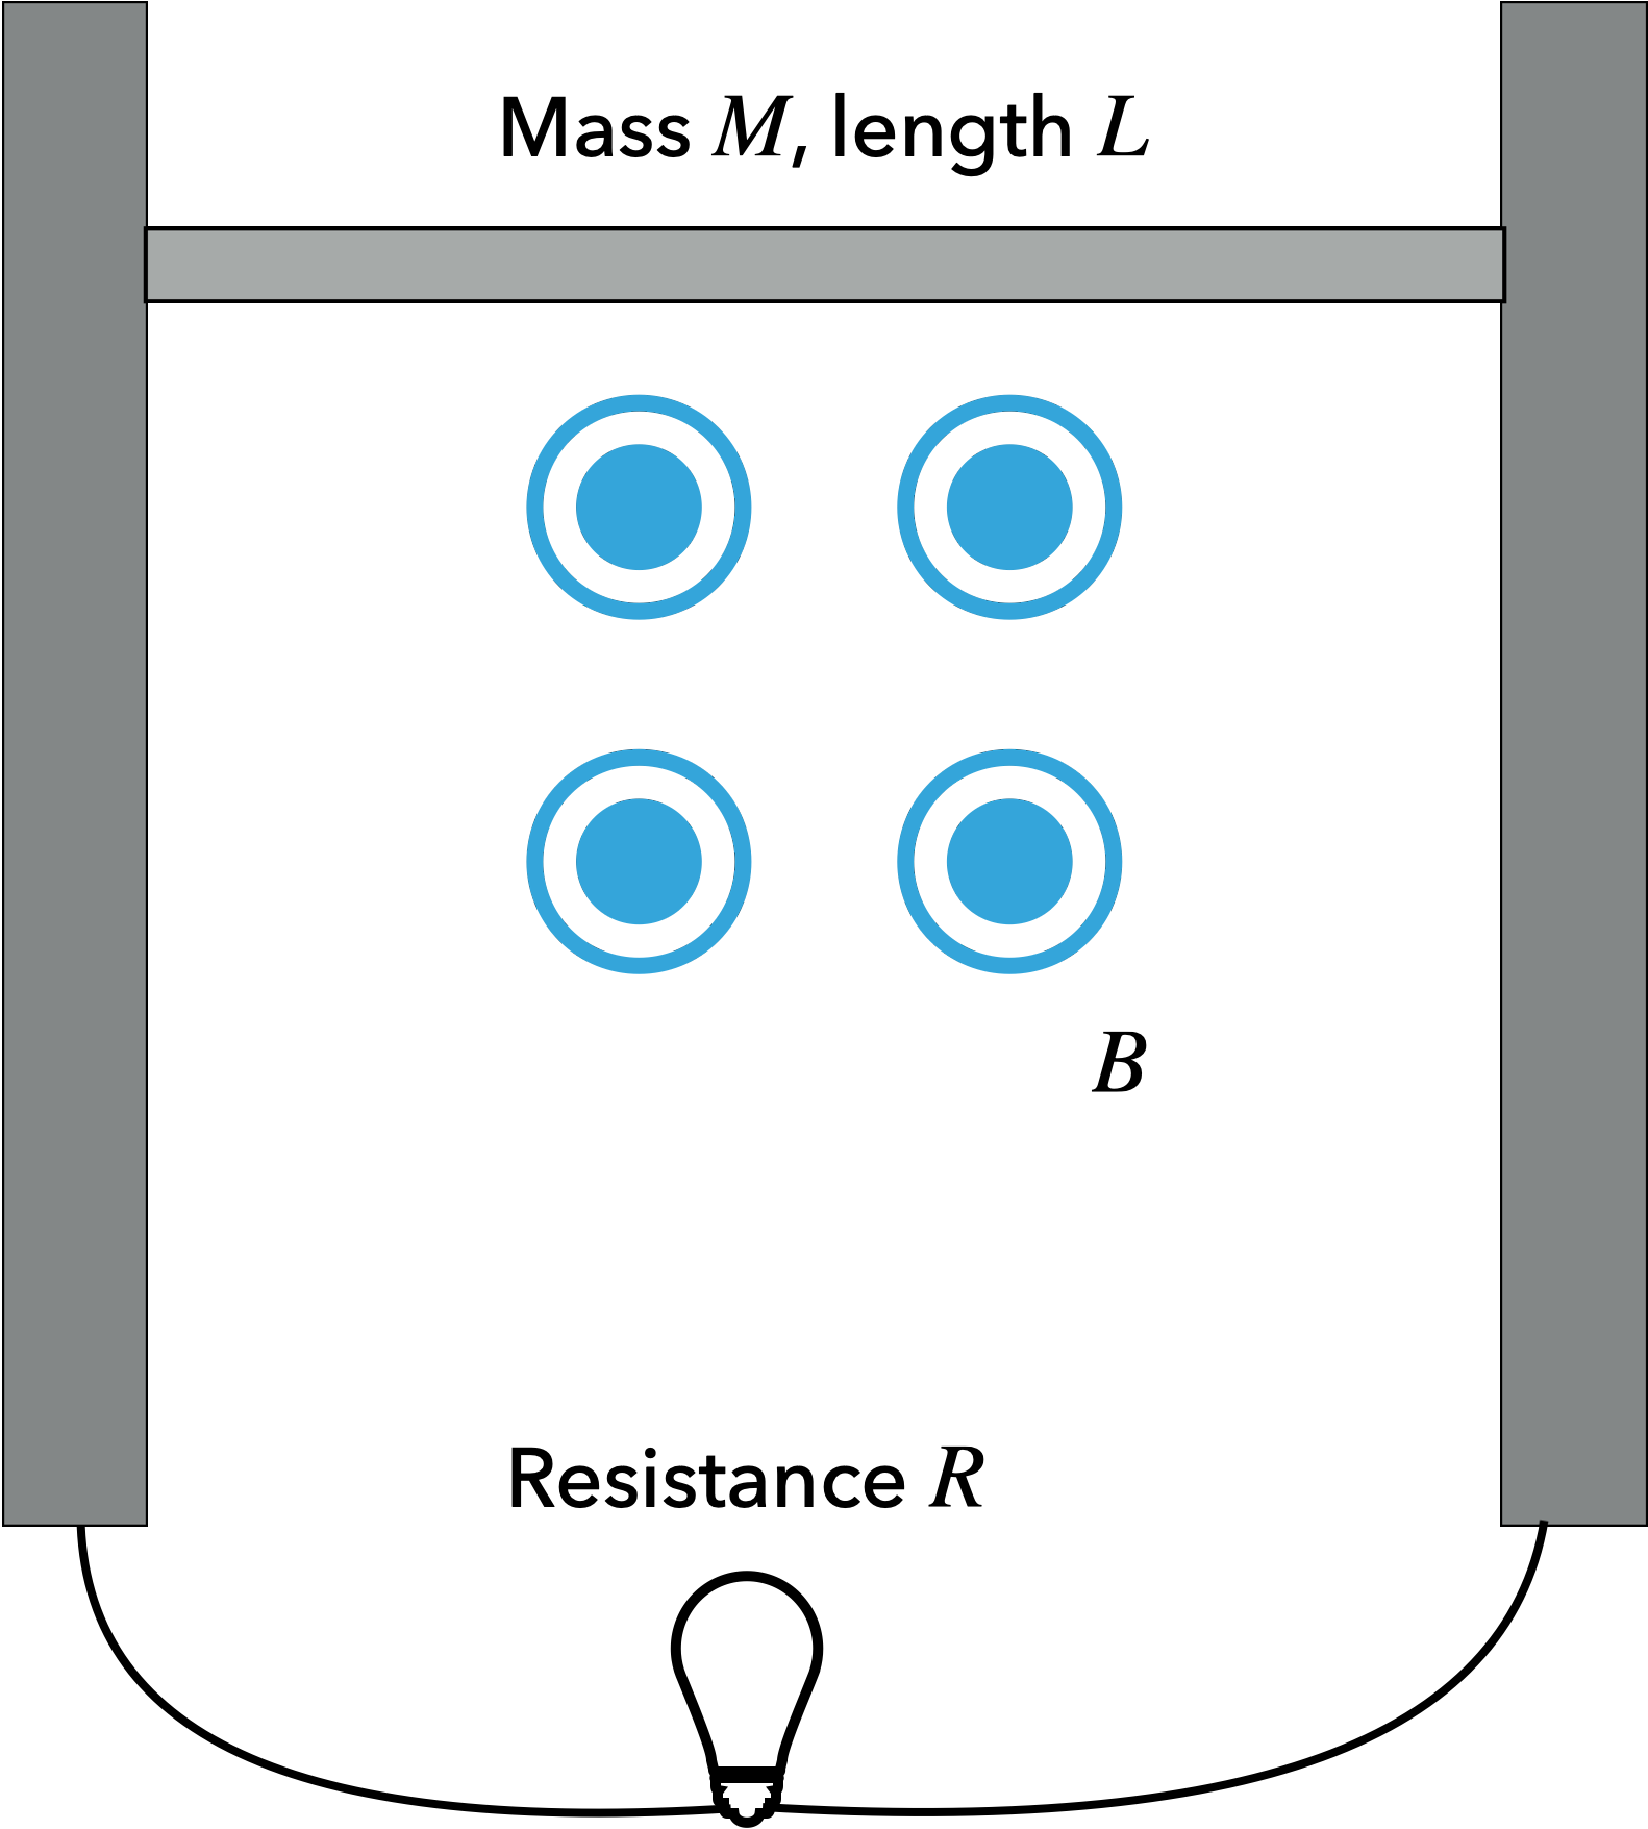
\includegraphics[width=.4\textwidth]{memf}
\end{center}


\begin{enumerate}
	\item What is the maximum speed of the metal bar?
	%\vspace{5 cm}
	\item How much power is dissipated through the light bulb once the bar reaches its maximum speed?
	%\vspace{5cm}
	\item What direction is the conventional current flowing through the light bulb as the bar travels with maximum speed? (Indicate on the diagram)

\end{enumerate}
\end{document}